\cleardoublepage
\chapter{Introduction}
%\markboth{Introduction}{Introduction}
%\addcontentsline{toc}{chapter}{Introduction}

Dark matter makes up most of the mass in galaxies and galaxy clusters and plays a crucial role in shaping cosmic structure. Despite decades of observational and theoretical effort, its fundamental nature remains one of the outstanding questions in physics and astronomy. At cosmological scales, dark matter halos form through gravitational collapse and hierarchical assembly, producing characteristic density profiles that encode information about the underlying dark matter model, assembly history, and internal dynamics.

Numerical simulations provide a controlled setting in which these processes can be studied. Interpreting the results requires care, because subtle trends may reflect genuine physics or arise from modelling choices and post-processing. The chapters that follow develop the theoretical background, describe the computational framework, and present the diagnostics and experiments used throughout this thesis.

\section{The cusp-core problem}

In standard Cold Dark Matter (CDM) cosmology, gravitational $N$-body simulations predict that dark matter halos develop steep, cuspy density profiles in their central regions, following a power-law slope $\gamma \approx -1.5$ to $-2$ within a characteristic transition radius. Observationally, however, many dwarf galaxies exhibit much shallower central profiles with slopes closer to $\gamma \approx -0.2$ to $-1$, a feature referred to as a density core. This discrepancy between the predicted cusps and observed cores, known as the \emph{cusp-core problem}, has motivated decades of investigation into whether the resolution lies in the nature of dark matter, the dynamical history of galaxies, or systematic observational uncertainties \citep{power2003inner}.

One promising explanation for core formation involves non-adiabatic perturbations to the potential. When supernovae, black hole feedback, or other energetic events suddenly alter the gravitational potential of a galaxy, orbits that were previously in equilibrium can be disrupted. Particles at small radii can then diffuse outward through repeated phase-space mixing, gradually flattening the inner density profile. More subtly, stochastic gravitational fluctuations generated by clumpy substructure or halo asymmetries can also transfer energy and angular momentum to central orbits over long dynamical times, producing a cumulative heating effect \citep{penarrubia2017fluctuations,penarrubia2019stochastic}. Such mechanisms appear particularly efficient in ultra-faint dwarf galaxies, which have shallow potential wells and are prone to ongoing tidal interactions.

\begin{figure}[H]
	\centering
	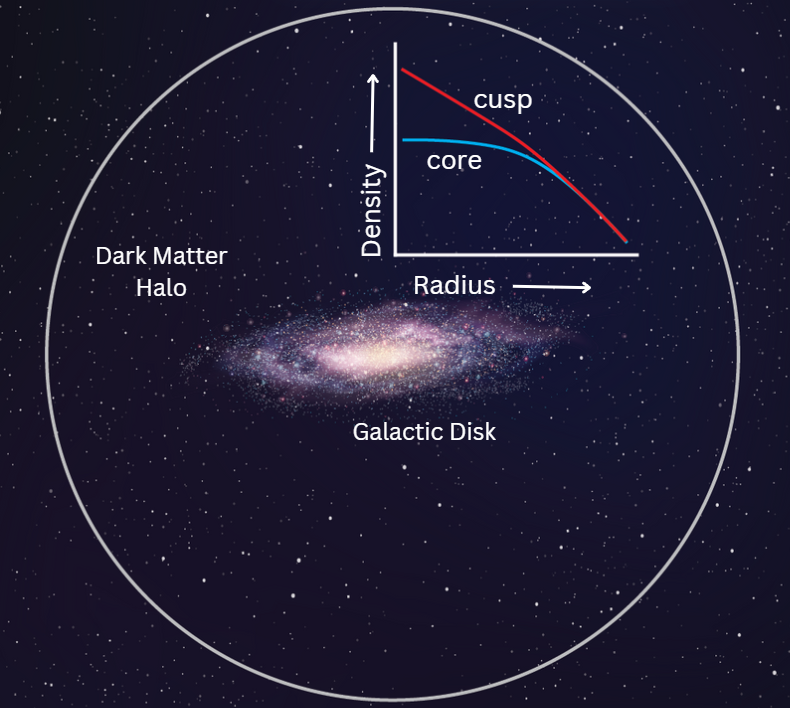
\includegraphics[width=0.7\textwidth]{content/ch1/img/cuspvcore.png}
	\caption{Cusp versus core density profiles. Image credit: AAS Nova (Down to the core: Dark matter deviations in ultra-faint dwarf galaxies) \citep{aasnova2024}.}
	\label{fig:intro_cusp_core}
\end{figure}

\section{Motivating question}

The persistent inner density decline observed in controlled, dark matter-only simulations of relaxed halos presents a puzzle. In such runs, there are no baryonic processes (supernovae, AGN feedback) and no time-dependent external perturbations. Gravity is purely Newtonian, computed with modern adaptive algorithms. Yet the simulated halos still exhibit a gradual flattening of their central profiles over time. This raises a critical question: is this decline a reflection of genuine collisionless dynamics, an artifact of numerical approximations in the gravity solver, or a side effect of the post-processing analysis pipeline?

If the observed density decline is primarily a numerical artifact, then the apparent core in simulations is unreliable and informs little about real galaxy evolution. If it is a genuine dynamical feature, then understanding its mechanism opens a window into collisionless relaxation and the role of global halo coupling.

This thesis focuses on determining which of these possibilities explains the persistent central density decline observed in a reference SWIFT simulation of a dark matter halo evolved in isolation over 100 Gyr.

\section{Aims and objectives}

The main goal of this work is to investigate the origin of the central density decline through controlled parameter studies and tests. The specific objectives are:

\begin{enumerate}

\item \textbf{Characterize the baseline behavior}: Establish what the reference simulation produces in terms of density profile evolution, and verify that the trend is robust against simple post-processing variations (centering method, snapshot noise reduction).

\item \textbf{Rule out trivial numerical explanations}: Test whether changes to numerical parameters significantly alter the observed decline. If numerical parameters prove insensitive, a more fundamental physical or structural process becomes more likely.

\item \textbf{Assess global and local influences}: Investigate whether the inner density trend reflects purely local physics or depends on the larger-scale halo environment.

\item \textbf{Evaluate the robustness of the effect}: Test whether the decline persists for different initial halo structures and different simulation volumes, to establish whether the mechanism is universal or tuning-dependent.

\end{enumerate}

The cumulative outcome will be either a validated mechanism (if the trend survives all tests and correlates with a specific physical process) or a ruled-out category of explanations.

\section{Thesis outline}

The thesis is organized as follows:

\begin{description}

\item[\textbf{Chapter 2: Theoretical background}] introduces the collisionless framework governing dark matter halos, defines the cusp-core phenomenology, and reviews the numerical considerations that affect halo simulations. This chapter establishes the theoretical minimum needed to interpret the results.

\item[\textbf{Chapter 3: Simulation model and implementation}] documents the numerical setup in detail. The SWIFT configuration, initial condition generation, halo parameter choices, and implementation details of the truncated-NFW model are described. This chapter is designed for reproducibility, a reader should be able to replicate the simulations and analysis from the information provided.

\item[\textbf{Chapter 4: Results and discussion}] presents the parameter studies and sensitivity analyses. The chapter progresses through five main tests: (i) the baseline evolution, (ii) box size sensitivity, (iii) initial condition dependence (cusp versus core), (iv) softening length variations, and (v) self-gravity solver parameter sensitivity. Each test is framed as a hypothesis to either support or eliminate candidate explanations. Later sections address shell contributions and hybrid models.

\item[\textbf{Chapter 5: Conclusions}] summarizes which explanations have been ruled out and which remain plausible, and outline suggestions for future work.

\end{description}

This thesis therefore focuses on determining whether the effect is numerical, methodological, or physical in origin, by combining targeted diagnostics with controlled variations of the numerical setup and initial conditions.
